\documentclass[a4paper]{article}
\usepackage{amsmath,amssymb,amsfonts,amsthm}
\usepackage{multicol}
\usepackage{multirow}
\usepackage{mathtools}
\usepackage{soul}
\usepackage{hyperref}
\hypersetup{
    colorlinks=true,
    linkcolor=blue,
    filecolor=magenta,      
    urlcolor=cyan,
    pdftitle={Overleaf Example},
    pdfpagemode=FullScreen,
    }
\usepackage{color}
\usepackage[table]{xcolor}
\usepackage[T1]{fontenc}
\usepackage{etoolbox}
\usepackage{multicol}
\usepackage{multirow}
\usepackage{fancyhdr}
\usepackage{graphicx}
\usepackage{array}
\usepackage{amsthm}
\usepackage{titlesec}
\usepackage{tikz}
\usetikzlibrary{arrows.meta,calc}
\renewcommand{\baselinestretch}{1.2}

\titleformat*{\section}{\large\bfseries}
\titleformat*{\subsection}{\normalsize\bfseries}

\graphicspath{{C:/Users/teoso/OneDrive/Documents/Tugas Kuliah/Template Math Depart/}}

\newtheorem{theorem}{Theorem}
\newtheorem*{teorema}{Teorema}
\newtheorem*{definisi}{Definisi}
\theoremstyle{definition}
\newtheorem*{bukti}{Bukti}

\newcommand{\Arg}{\text{Arg}}

\begin{document}
\fancyhead[L]{\textit{Teosofi Hidayah Agung}}
\fancyhead[R]{\textit{5002221132}}
\pagestyle{fancy}
\section*{Nomor 4}
  \noindent Diberikan \( X = \{ z \in \mathbb{C} : |z| = 1 \} \), yaitu lingkaran dengan pusat titik \( 0 \) dan berjari-jari \( 1 \) pada bidang kompleks. Untuk sebarang \( z, w \in X \) didefinisikan $\rho(z,w)=0$ jika  $z = w$,
    $\rho(z,w)=\pi$ jika $z = -w$, dan $\rho(z,w)$ menyatakan panjang busur terpendek yang menghubungkan $z$ dan $w$ jika  $z \neq \pm w$. Buktikan bahwa \( \rho \) merupakan metrik pada \( X \). 
  \begin{bukti}
    Dari informasi pada soal, didapatkan ilustrasi sebagai berikut
    \begin{center}
      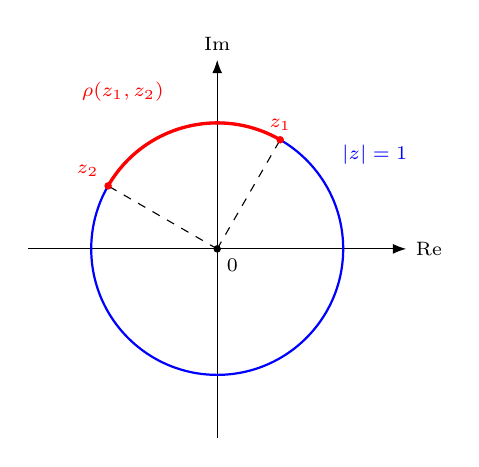
\begin{tikzpicture}[scale=0.8]
        \draw[-Latex] (-3,0) -- (3,0) node[right] {\scriptsize Re};
        \draw[-Latex] (0,-3) -- (0,3) node[above] {\scriptsize Im};
        \draw[thick,blue] (0,0) circle (2);
        \node[blue] (z) at (2.5,1.5) {\scriptsize$|z|=1$};
        \node[red] (z') at (-1.5,2.5) {\scriptsize$\rho(z_1,z_2)$};
        \draw[fill] (0,0) circle (0.05) node[below right] (z'') at (0,0) {\scriptsize$0$};
        \draw[dashed] (0,0) -- ($(0,0) + (150:2)$);
        \draw[dashed] (0,0) -- ($(0,0) + (60:2)$);
        \draw[red,fill] ($(0,0) + (60:2)$) circle (0.05) node[above]{\scriptsize$z_1$}; 
        \draw[red,fill] ($(0,0) + (150:2)$) circle (0.05) node[above left]{\scriptsize$z_2$}; 
        \draw[very thick,red] ($(0,0) + (60:2)$) arc (60:150:2);
      \end{tikzpicture}
      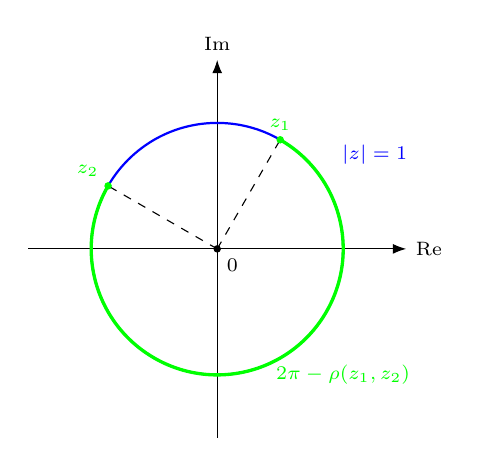
\begin{tikzpicture}[scale=0.8]
        \draw[-Latex] (-3,0) -- (3,0) node[right] {\scriptsize Re};
        \draw[-Latex] (0,-3) -- (0,3) node[above] {\scriptsize Im};
        \draw[thick,blue] (0,0) circle (2);
        \node[blue] (z) at (2.5,1.5) {\scriptsize$|z|=1$};
        \node[green] (z') at (2,-2) {\scriptsize$2\pi-\rho(z_1,z_2)$};
        \draw[fill] (0,0) circle (0.05) node[below right] (z'') at (0,0) {\scriptsize$0$};
        \draw[dashed] (0,0) -- ($(0,0) + (150:2)$);
        \draw[dashed] (0,0) -- ($(0,0) + (60:2)$);
        \draw[green,fill] ($(0,0) + (60:2)$) circle (0.05) node[above]{\scriptsize$z_1$}; 
        \draw[green,fill] ($(0,0) + (150:2)$) circle (0.05) node[above left]{\scriptsize$z_2$}; 
        \draw[very thick,green] ($(0,0) + (150:2)$) arc (150:420:2);
      \end{tikzpicture}
    \end{center} 
    Sehingga untuk \( z, w \in X \) panjang busur terpendek dapat dirumuskan sebagai
    \begin{equation*}
      \rho(z,w) = \min\left\{ \left|\Arg(z)-\Arg(w)\right|, 2\pi - \left|\Arg(z) - \Arg(w)\right|\right\},\quad z,w \in X
    \end{equation*} 
    yang dimana telah memenuhi ketentuan fungsi $\rho$ yang diberikan pada soal.

    Selanjutnya akan dibuktikan bahwa \(\rho\) memenuhi sifat-sifat metrik.
    \begin{enumerate}
      \item \textbf{(Positifitas)} Ambil sebarang \( z, w \in X \) maka jelas berlaku 
      \begin{align*}
        |\Arg(z) - \Arg(w)| \geq 0
      \end{align*}
      dan karena $\Arg(z),\Arg(w) \in [-\pi,\pi]$, akibatnya 
      \begin{align*}
        |\Arg(z) - \Arg(w)| &\leq 2\pi\\
        2\pi - |\Arg(z) + \Arg(w)| &\geq 0.
      \end{align*}
      Jadi \(\rho(z,w) \geq 0\). 
      \item Akan dibuktikan bahwa \(\rho(z,w) = 0 \iff z = w\). 
      \begin{itemize}
        \item (\(\Leftarrow\)) Terbukti dari definisi \(\rho(z,w)\).
        \item (\(\Rightarrow\)) Ambil $z,w\in X$ dan misalkan \( \rho(z,w) = 0 \), maka berlaku
        \begin{align*}
          \min\left\{ \left|\Arg(z)-\Arg(w)\right|, 2\pi - \left|\Arg(z) - \Arg(w)\right| \right\} = 0
        \end{align*}
        Berarti \(|\Arg(z) - \Arg(w)|=0\) atau \(2\pi - |\Arg(z) - \Arg(w)| = 0\). 
        \begin{itemize}
          \item Jelas untuk \(|\Arg(z) - \Arg(w)|=0\) berakibat \(\Arg(z) = \Arg(w)\) dan \(z = w\).
          \item Untuk \(2\pi - |\Arg(z) - \Arg(w)| = 0\) berlaku \(\Arg(z) - \Arg(w) = 2\pi\) ($2\pi$ atau $-2\pi$ sama saja untuk bilangan kompleks). Selanjutnya perhatikan bahwa
          \begin{align*}
            \exp\left[i(\Arg(z)-\Arg(w))\right] &= \exp(2\pi i)\\
            \exp(i\Arg(z))\exp(-i\Arg(w)) &= 1\\
            |z|e^{i\Arg(z)}|w|e^{-i\Arg(w)} &= 1\\
            z\overline{w} &= 1\\
            z&= \frac{1}{\overline{w}}
          \end{align*}
          Karena $|w|=1$ berakibat $w=\dfrac{1}{\overline{w}}$ sehingga $z=w$.
        \end{itemize}
      \end{itemize}
      Jadi \(\rho(z,w) = 0 \iff z = w\). 
      \item \textbf{(Simetri)} Untuk setiap \( z, w \in X \) berlaku bahwa 
      \begin{align*}
        \rho(z,w)&=\min\left\{ \left|\Arg(z)-\Arg(w)\right|, 2\pi - \left|\Arg(z) - \Arg(w)\right| \right\} \\
        &= \min\left\{ \left|\Arg(w)-\Arg(z)\right|, 2\pi - \left|\Arg(w) - \Arg(z)\right| \right\}\\
        &=\rho(w,z)
      \end{align*}
      Jadi \(\rho(z,w) = \rho(w,z)\).
      
      \item \textbf{(Ketaksamaan Segitiga)} Misalkan \( z, w, v \in X \) dan akan dibuat menjadi dua kasus.
      \begin{itemize}
        \item Untuk $\Arg(z) \leq \Arg(v) \leq \Arg(w)$, dapat diilustrasikan sebagai berikut
        \begin{center}
          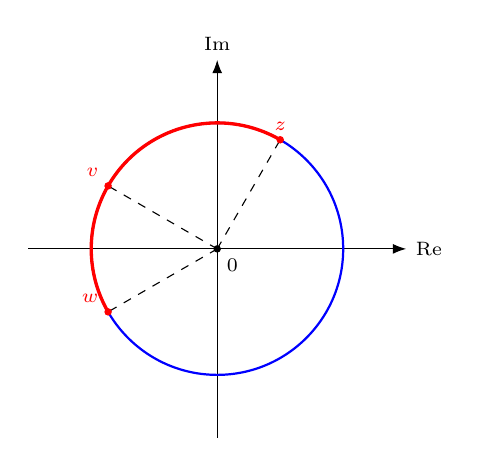
\begin{tikzpicture}[scale=0.8]
            \draw[-Latex] (-3,0) -- (3,0) node[right] {\scriptsize Re};
            \draw[-Latex] (0,-3) -- (0,3) node[above] {\scriptsize Im};
            \draw[thick,blue] (0,0) circle (2);
            \node[blue] (z) at (2.5,1.5) {};
            \node[red] (z') at (-1.5,2.5) {};
            \draw[fill] (0,0) circle (0.05) node[below right] (z'') at (0,0) {\scriptsize$0$};
            \draw[dashed] (0,0) -- ($(0,0) + (150:2)$);
            \draw[dashed] (0,0) -- ($(0,0) + (210:2)$);
            \draw[dashed] (0,0) -- ($(0,0) + (60:2)$);
            \draw[red,fill] ($(0,0) + (60:2)$) circle (0.05) node[above]{\scriptsize$z$}; 
            \draw[red,fill] ($(0,0) + (150:2)$) circle (0.05) node[above left]{\scriptsize$v$}; 
            \draw[red,fill] ($(0,0) + (210:2)$) circle (0.05) node[above left]{\scriptsize$w$}; 
            \draw[very thick,red] ($(0,0) + (60:2)$) arc (60:210:2);
          \end{tikzpicture}
        \end{center}
        Dari ilustrasi diatas berlaku
        \[\rho(z,w) = \rho(z,v) + \rho(v,w)\]
        \item Tanpa mengurangi keumuman, misalkan $\Arg(z) \leq \Arg(w) \leq \Arg(v)$ diilustrasikan sebagai berikut
        \begin{center}
          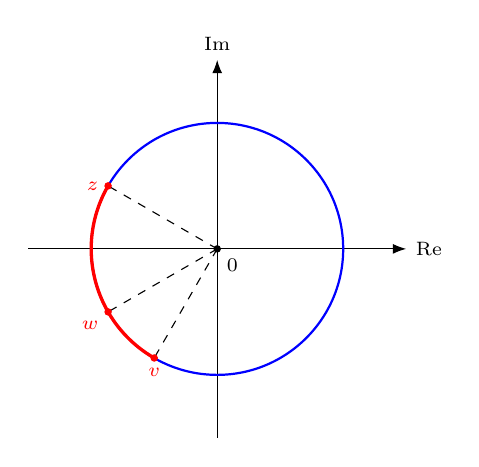
\begin{tikzpicture}[scale=0.8]
            \draw[-Latex] (-3,0) -- (3,0) node[right] {\scriptsize Re};
            \draw[-Latex] (0,-3) -- (0,3) node[above] {\scriptsize Im};
            \draw[thick,blue] (0,0) circle (2);
            \node[blue] (z) at (2.5,1.5) {};
            \node[green] (z') at (2,-2) {};
            \draw[fill] (0,0) circle (0.05) node[below right] (z'') at (0,0) {\scriptsize$0$};
            \draw[dashed] (0,0) -- ($(0,0) + (240:2)$);
            \draw[dashed] (0,0) -- ($(0,0) + (210:2)$);
            \draw[dashed] (0,0) -- ($(0,0) + (150:2)$);
            \draw[red,fill] ($(0,0) + (150:2)$) circle (0.05) node[left]{\scriptsize$z$}; 
            \draw[red,fill] ($(0,0) + (210:2)$) circle (0.05) node[below left]{\scriptsize$w$}; 
            \draw[red,fill] ($(0,0) + (240:2)$) circle (0.05) node[below]{\scriptsize$v$}; 
            \draw[very thick,red] ($(0,0) + (150:2)$) arc (150:240:2);
          \end{tikzpicture}
        \end{center}
        Dari ilustrasi diatas berlaku
        \[\rho(z,w) \leq \rho(z,v) + \rho(v,w)\]
      \end{itemize}
      Jadi \(\rho(z,w) \leq \rho(z,v) + \rho(v,w)\) dengan kesamaan terjadi ketika titik $v$ berada diantara busur terpendek $z$ dan $w$. 
    \end{enumerate}
    $\therefore$ \(\rho\) merupakan metrik pada \(X\). \(\square\)
  \end{bukti}
\end{document}